\documentclass[11pt,a4paper]{article}
\usepackage[hyperref]{naaclhlt2019}
% ---------- Packages (simple + student-friendly) ----------
\usepackage[margin=1in]{geometry}
\usepackage{graphicx}
\usepackage{amsmath,amssymb,amsfonts}
\usepackage{booktabs}
\usepackage{hyperref}
\usepackage{enumitem}
\usepackage{caption}
\usepackage{float}
\usepackage{microtype}

\aclfinalcopy 

\hypersetup{
  colorlinks=true,
  linkcolor=blue,
  urlcolor=blue,
  citecolor=blue
}

\setlength{\parindent}{0pt}
\setlength{\parskip}{6pt}

% ---------- Fill these in ----------
\newcommand{\coursename}{DATA 2010}
\newcommand{\termname}{Winter 2026} % change if needed
\newcommand{\duedate}{[DUE DATE, 11:59pm]} % fill in
\newcommand{\submissionplace}{UM Learn} % change if needed

\title{\textbf{DATA 2010:\\ Predicting State-Level Residential Energy Consumption}\\
\large \termname}
\author{
Spencer Brule (8025008) \\
}
\date{}

\begin{document}
\maketitle
% =========================================================
\section{Project Overview}
Record-breaking energy demands, combined with growing energy conservation initiatives, highlight the importance of developing models that can reliably predict and inform the allocation of energy resources. As populations grow and climate patterns become increasingly variable, the ability to anticipate energy needs becomes both economically and environmentally significant. In this project, we investigate the extent to which publicly available weather data can be used to model and predict residential energy consumption across the United States.
Specifically, this work leverages data obtained from the U.S. Energy Information Administration (EIA), which provides approximately twenty years of monthly, state-level records for residential natural gas consumption (measured in million cubic feet, MMCF) and electricity consumption (measured in million kilowatt-hours, Mkh). This dataset is paired with weather data acquired from OpenMeteo API, which offers flexibility in feature location, and date selection. With additional feature engineering, most notably Heating Degree Days (HDD) and Cooling Degree Days (CDD), which serve as widely accepted proxies for temperature-driven energy demand, these datasets aligning to explore both explanatory and predictive relationships between weather conditions and energy usage. From an exploratory standpoint, understanding how strongly HDD and CDD correlate with natural gas and electricity consumption, respectively, provides insight into seasonal consumption patterns and the extent to which weather alone can explain observed variability. From a predictive standpoint, the project evaluates whether these relationships can be leveraged to construct models that generalize well across time and across different states.
To achieve this, multiple modeling approaches will be considered, including linear regression models and more flexible, non-linear tree-based methods such as Random Forest. Linear models offer interpretability and simplicity, making them attractive for understanding direct relationships between variables. In contrast, tree-based models are capable of capturing complex interactions and non-linear effects, which may be present due to various hidden factors which influence energy consumption. 

Accurate forecasting of residential energy requirements, both in electricity and natural gas, has broad implications in state-level resource planning and infrastructure investment/development. The ability to anticipate demand can allow the energy sector to efficiently allocate resources and minimize waste. Furthermore, the ability to forecast spikes in demand can inform regulators and avoid energy shortages. 

By answering these questions, this project contributes tangible value in a lightweight and open-source model. This project details a successful approach to predicting both natural gas and electricity consumption by state. In addition to accurate predictions, it is shown that a tree based model outperforms linear models given our data and that heating and cooling degree days have strong explanatory power when it comes to energy consumption.


% =========================================================
\pagebreak
\section{Research Questions}
This paper seeks to address the following research questions:
\begin{enumerate}
\item To what extent are heating degree days and cooling degree days correlated to natural gas and electricity consumption, respectively?
\item Does a linear model outperform tree-based models, or do non-linear methods provide a significant advantage?
\item Can state-level electricity and natural gas consumption be accurately predicted based on weather data alone, or are additional infrastructure, socioeconomic and structural factors required to achieve strong predictive performance?
\end{enumerate}

% =========================================================
\section{Data Source and Description}

\subsection{Data Origin}
\begin{itemize}
  \item Dataset name: \href{https://open-meteo.com/en/docs/historical-weather-api}{OpenMeteo API}
  \item What each row represents: Summary weather results from a single day at a single location (State)
  \item Key columns: Date, Min Temp, Mean Temp, Max Temp, Daylight Duration, Wind speed, Wind gusts, Radiation, Precipitation
\end{itemize}
\begin{itemize}[leftmargin=18pt]
  \item Dataset name: \href{https://www.eia.gov/opendata/browser/natural-gas}{EIA API (Gas)}, \href{https://www.eia.gov/opendata/browser/electricity}{EIA API (Electricity)}
  \item What each row represents: Monthly summary totals for state-level energy consumption, sales, consumers, residential and industry data.
  \item Key columns: Period (Date), State, Consumption
\end{itemize}

\subsection{Basic dataset facts}
\begin{center}
EIA(Electricity)
\begin{tabular}{ll}
\toprule
Number of rows & [111600] \\
Number of columns & [11] \\
Time range (Monthly) & [2001-2026] \\
Missing values present? & [Yes, Imputed] \\
\bottomrule
\end{tabular}
\end{center}
\begin{center}
EIA(Gas)
\begin{tabular}{ll}
\toprule
Number of rows & [104651] \\
Number of columns & [11] \\
Time range (Monthly) & [2001-2026] \\
Missing values present? & [No] \\
\bottomrule
\end{tabular}
\end{center}
\begin{center}
OpenMeteo(Weather)
\begin{tabular}{ll}
\toprule
Number of rows & [465681] \\
Number of columns & [12] \\
Time range (Daily) & [2001-2026] \\
Missing values present? & [No] \\
\bottomrule
\end{tabular}
\end{center}

% =========================================================
\section{Data Cleaning and Feature Engineering}

\subsection{Energy Data}
Using the Energy Information Administration(EIA) API, datasets for electricity and natural gas consumption by state were downloaded. These datasets were complete and required minimal cleaning; such as trimming, date decomposition, and minor imputation. \newline
For each energy dataset, industrial and commercial consumer entries were removed as they are not a focus of this model. Further trimming eliminated unnecessary features leaving the dataset with only date, state, and total endpoint consumption of either type of energy. Select rows which contained inaccurate states such as "U.S." or "D.C." were dropped since they don't match the other data and don't align with the goal of the model.  Features were renamed with units of measurement to save space and persist units. For model performance and compatibility with other data, the 'date' column was decomposed into 'year' and 'month' features. Missing values were detected and imputed in approximately 0.12\% of electricity records. \newline
Imputation for our target variable(s) relies on an understanding of the behaviour; since average consumption for winter months is dissimilar from average consumption for summer months, simply imputing the mean would lead to poor imputation. Additionally, as state populations grow (or shrink) over time, an average of twenty-five years may also lead to inaccurate imputation. Therefore, the simple solution of imputing the previous year's value for that state and month was employed.\newline
For electricity and gas data, normalization of the target features (Mkh, MMCF) by the residential population was considered and avoided due to unavailability of gas consumer population. Electricity customers could serve as a proxy for gas customers since both datasets are residential and belong to the same state; however, a conscious choice was made to allow the model to handle these values without normalization.
The resulting concatenated energy dataframe includes 5 features:
Year, Month, State, MMCF (Gas Consumption), Mkh (Electricity Consumption).

\subsection{Weather Data}

Interacting with the OpenMeteo Weather API provided many advantages, namely the ability to select from a large range of potential features, the ability to define date ranges for these features, and the completeness of the data (no missing values). Of the 30+ available features, a subset of 8 features were chosen with an additional 2 being engineered. Features were selected based on relevance to residential household temperature control and by proxy, electricity/gas consumption. These features included:

\begin{center}
Weather Feature Selection \\
(Table 4.1)\\
\begin{tabular}{ll}
\toprule
Feature & Aggregation \\
&Strategy\\
\midrule
Min Temperature (C)& Minimum\\
Mean Temperature (C)& Mean\\
Max Temperature (C)& Maximum\\
Daylight Duration (sec)& Mean\\
Wind speed (kph)& Mean\\
Wind gusts (kph)& Mean\\
Radiation (MJm2)& Sum\\
Precipitation (mm)& Sum\\
(Eng.)Heating Degree Days& Sum\\
(Eng.)Cooling Degree Days& Sum\\
\bottomrule
\end{tabular}
\end{center}
\begin{figure}
    \centering
    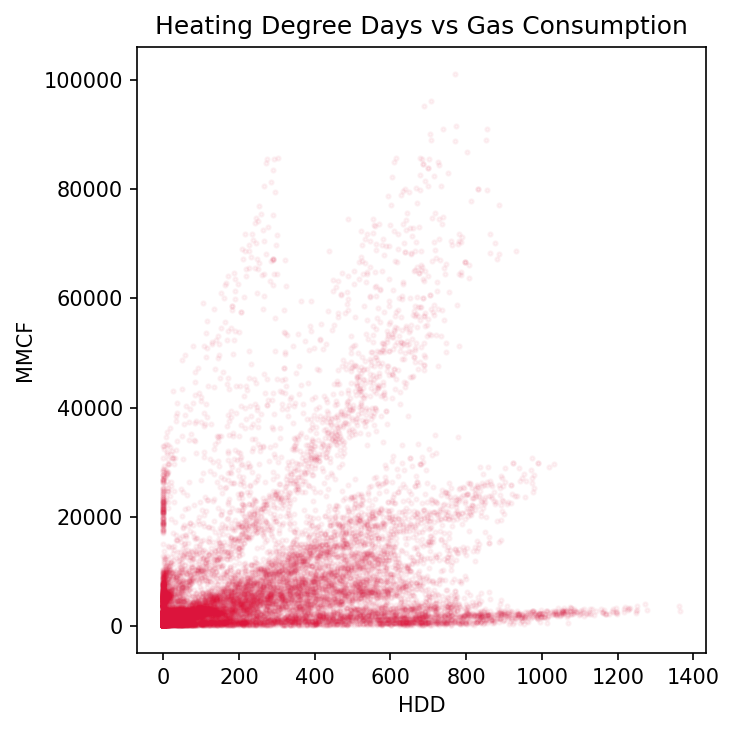
\includegraphics[width=\columnwidth]{HDDvsGas.png}
    \caption{Relationship between HDD and Gas consumption}
    \label{fig: 4.2}
\end{figure}

\begin{figure}
    \centering
    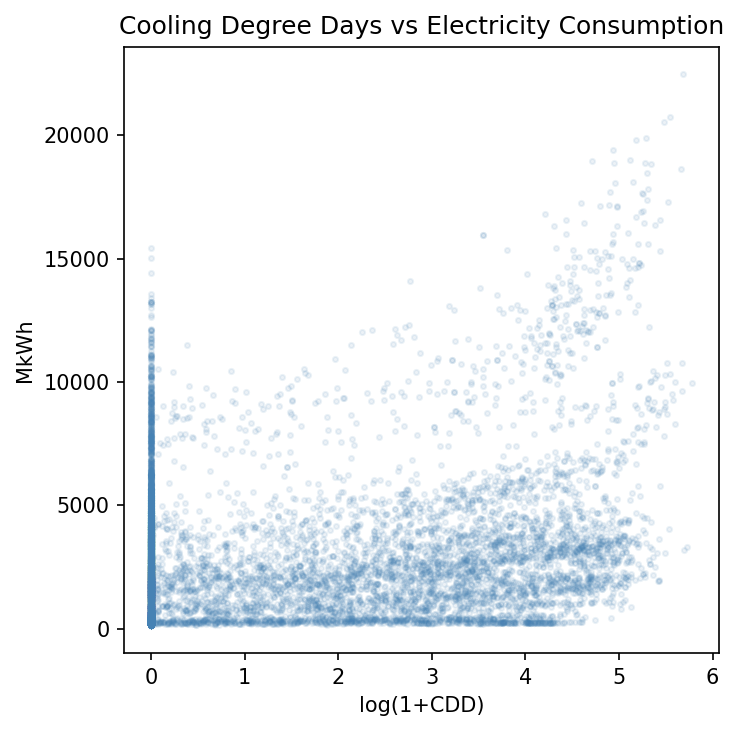
\includegraphics[width=\columnwidth]{CDDvsElectricity.png}
    \caption{Relationship between CDD and Electricity consumption}
    \label{fig: 4.3}
\end{figure}

\subsection{Feature Engineering}
For each state, the granularity of entries for weather data was finer than that of the energy data. This provided an excellent opportunity to engineer features prior to eventual aggregation to match the granularity of the two data frames. Aggregation of days by month for each feature was based on the strategy outlined in table 4.1. \\
Given the goal of attempting to measure energy consumption based on weather, feature engineering was employed to manufacture two new features: 'Heating Degree Days' and 'Cooling Degree Days'. The objective of these features is to apply a metric to days in which the weather dictates the requirement for heating or cooling of the household. Based on the recommended indoor temperatures outlined by the World Health Organization (WHO), our model uses a household temperature range between $17.8$ to $23.9$ celsius[1], average daily temperatures above this range indicate a requirement for cooling, and temperatures below, heating.  
$$
HDD = 
\begin{cases}
17.8 - T_{avg}, & \text{if } T_{avg} < 17.8 \\
0, & \text{otherwise}\\
\end{cases}
$$
$$
CDD =
\begin{cases}
T_{avg}  - 23.9, & \text{if } T_{avg} > 23.9\\
0, & \text{otherwise}
\end{cases}
$$
\textit{where $T_{avg}$ is the average daily temperature.}

Implementing this formula, two new features are generated which effectively capture not only the need for heating or cooling, but quantify the severity of difference in outdoor temperature versus indoor climate control. We can see that HDD exhibit strong explanatory power for gas consumption (Fig \ref{fig: 4.2}.); however CDD, while showing some correlation, reveal unexplained increases in electricity consumption where CDD is zero, suggesting the presence of additional influencing factors(Fig \ref{fig: 4.3}.).

%Electricity vs month
\begin{figure}
    \centering
    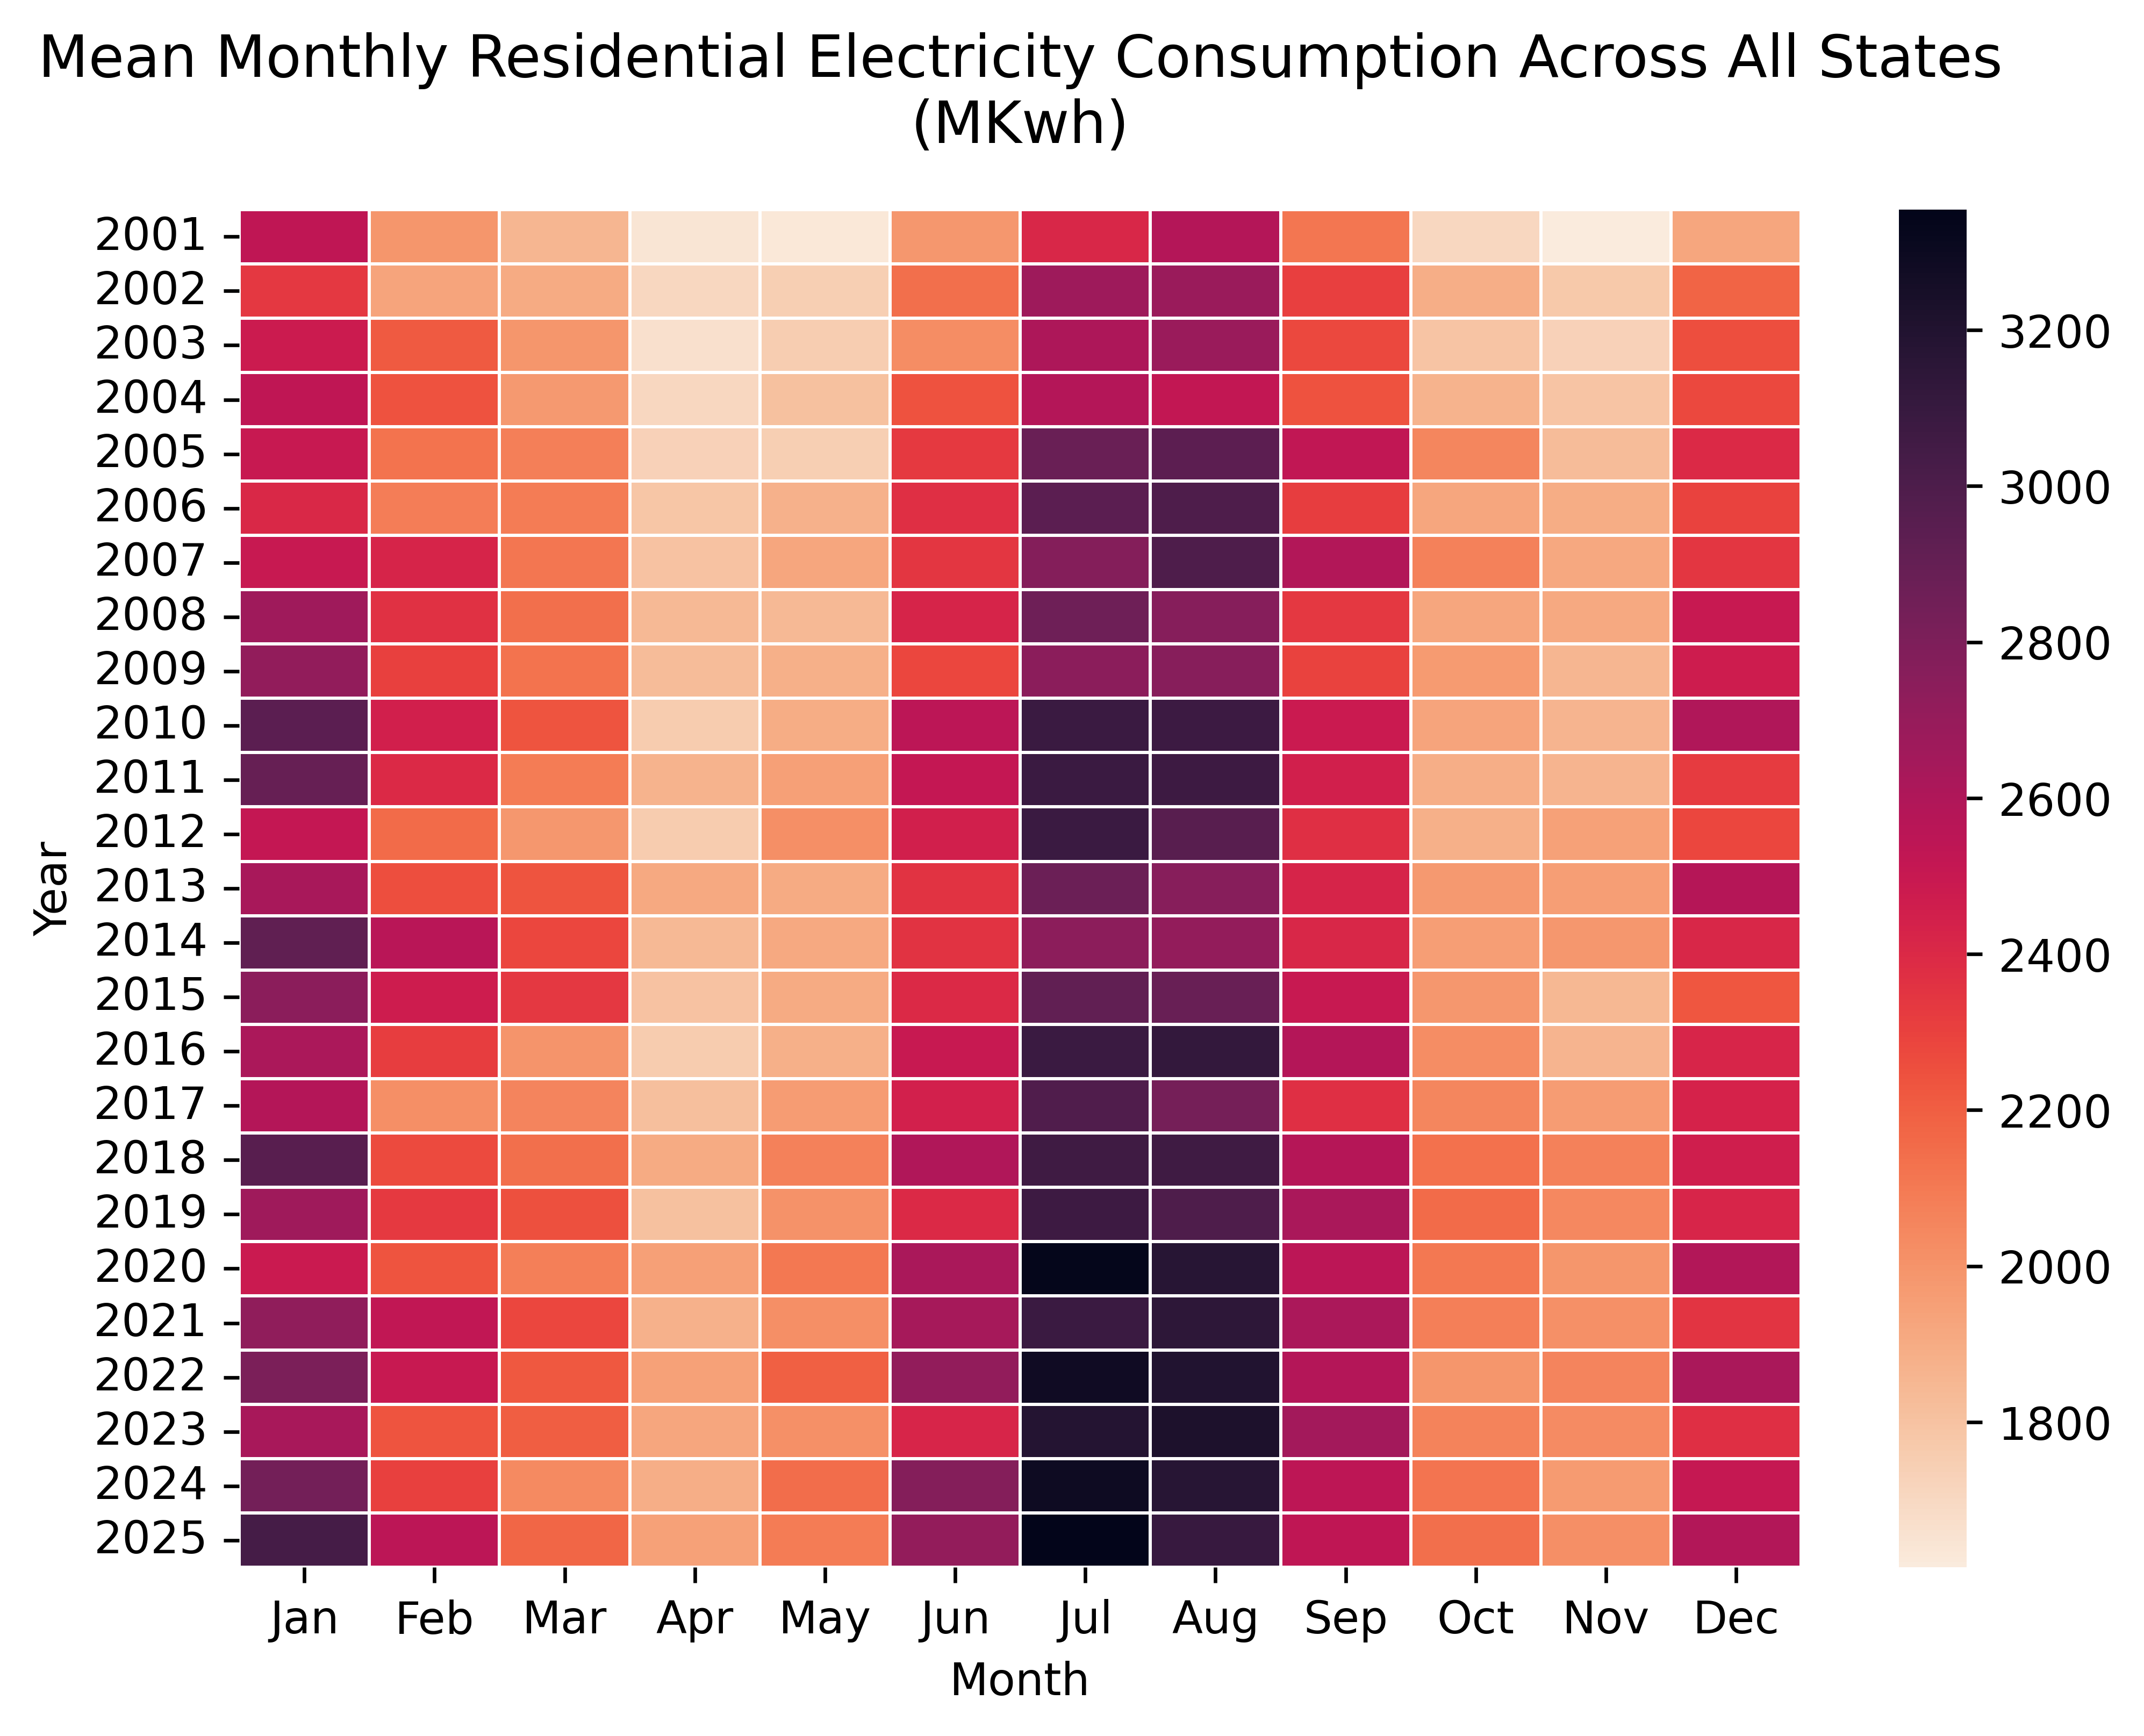
\includegraphics[width=\columnwidth]{electricityConsump.png}
    \caption{Dual peak annual electricity consumption}
    \label{fig: 5.2}
\end{figure}

\section{Encoding}
Feature encoding is an important aspect of setting up data for use in a machine learning model. By transforming categorical data into numerical values, it allows the model to extract information in an intuitive manner. The following two methods were used for feature encoding:
\begin{enumerate}
    \item \textbf{One Hot Encoding} - States\\
        The State column was divided into 50 features representing each state and each with a binary value whether or not that entry belongs to that state. Intuitively, the following formula holds: 
        $$
        \sum_{i=1}^{50}State_i = 1, \text{ for each observation}
        $$
    \item \textbf{Cyclical Encoding} - Months\\
        In the context of this model, months represent the changing of seasons and temperatures more so than the passage of time. To avoid the linear representation of months (01-12), we employ cyclical-type encoding, mapping months to x,y cartesian coordinates representing each month in a circle using the following formula.
        $$
        x = \sin{\left(\frac{2 \pi M}{12}\right)}\\
        $$
        $$
        y = \cos{\left(\frac{2 \pi M}{12}\right)}\\
        $$
        \textit{where M = month, representing the numerical value of each month (eg. April = 04).}
\end{enumerate}
With the completion of encoding, the data set is ready for use in a model.

% =========================================================
\section{Exploratory Data Analysis and Visualization}
%Temp
\begin{figure*}[t]
    \centering
    \includegraphics[width=1\textwidth]{gasvstemp.png}
    \caption{Inverse relationship between gas consumption and temperature}
    \label{fig: 5.1}
\end{figure*}


Our EDA will serve to illustrate and confirm some basic assumptions about our data as well as offering more in-depth insights into their correlations and inform strategies moving forward.

Firstly, our initial and seemingly trivial observation from HDD is that natural gas consumption and temperature have a strong negative correlation - that is to say generally, when temperature decreases, gas consumption increase and vice-versa. Taking a sample from Illinois(Fig \ref{fig: 5.1}.), we see this assumption confirmed.

Additionally, based on our observations of correlations between CDD and electricity consumption, we see a somewhat expected result; we see spikes in electricity consumption in summer months (Jul, Aug) and in winter months (Dec, Jan, Feb). (Fig \ref{fig: 5.2}.) Not only does this support the existence of additional hidden factors influencing electricity consumption, but also illustrates that these factors are seemingly influencing winter months more than others. 



Plotting our selected features into a correlation heatmap (Fig \ref{fig: 5.3}.) allows us to make valuable insights into linear relationships between variables. \newline
%Correlation Heatmap
\begin{figure}
    \centering
    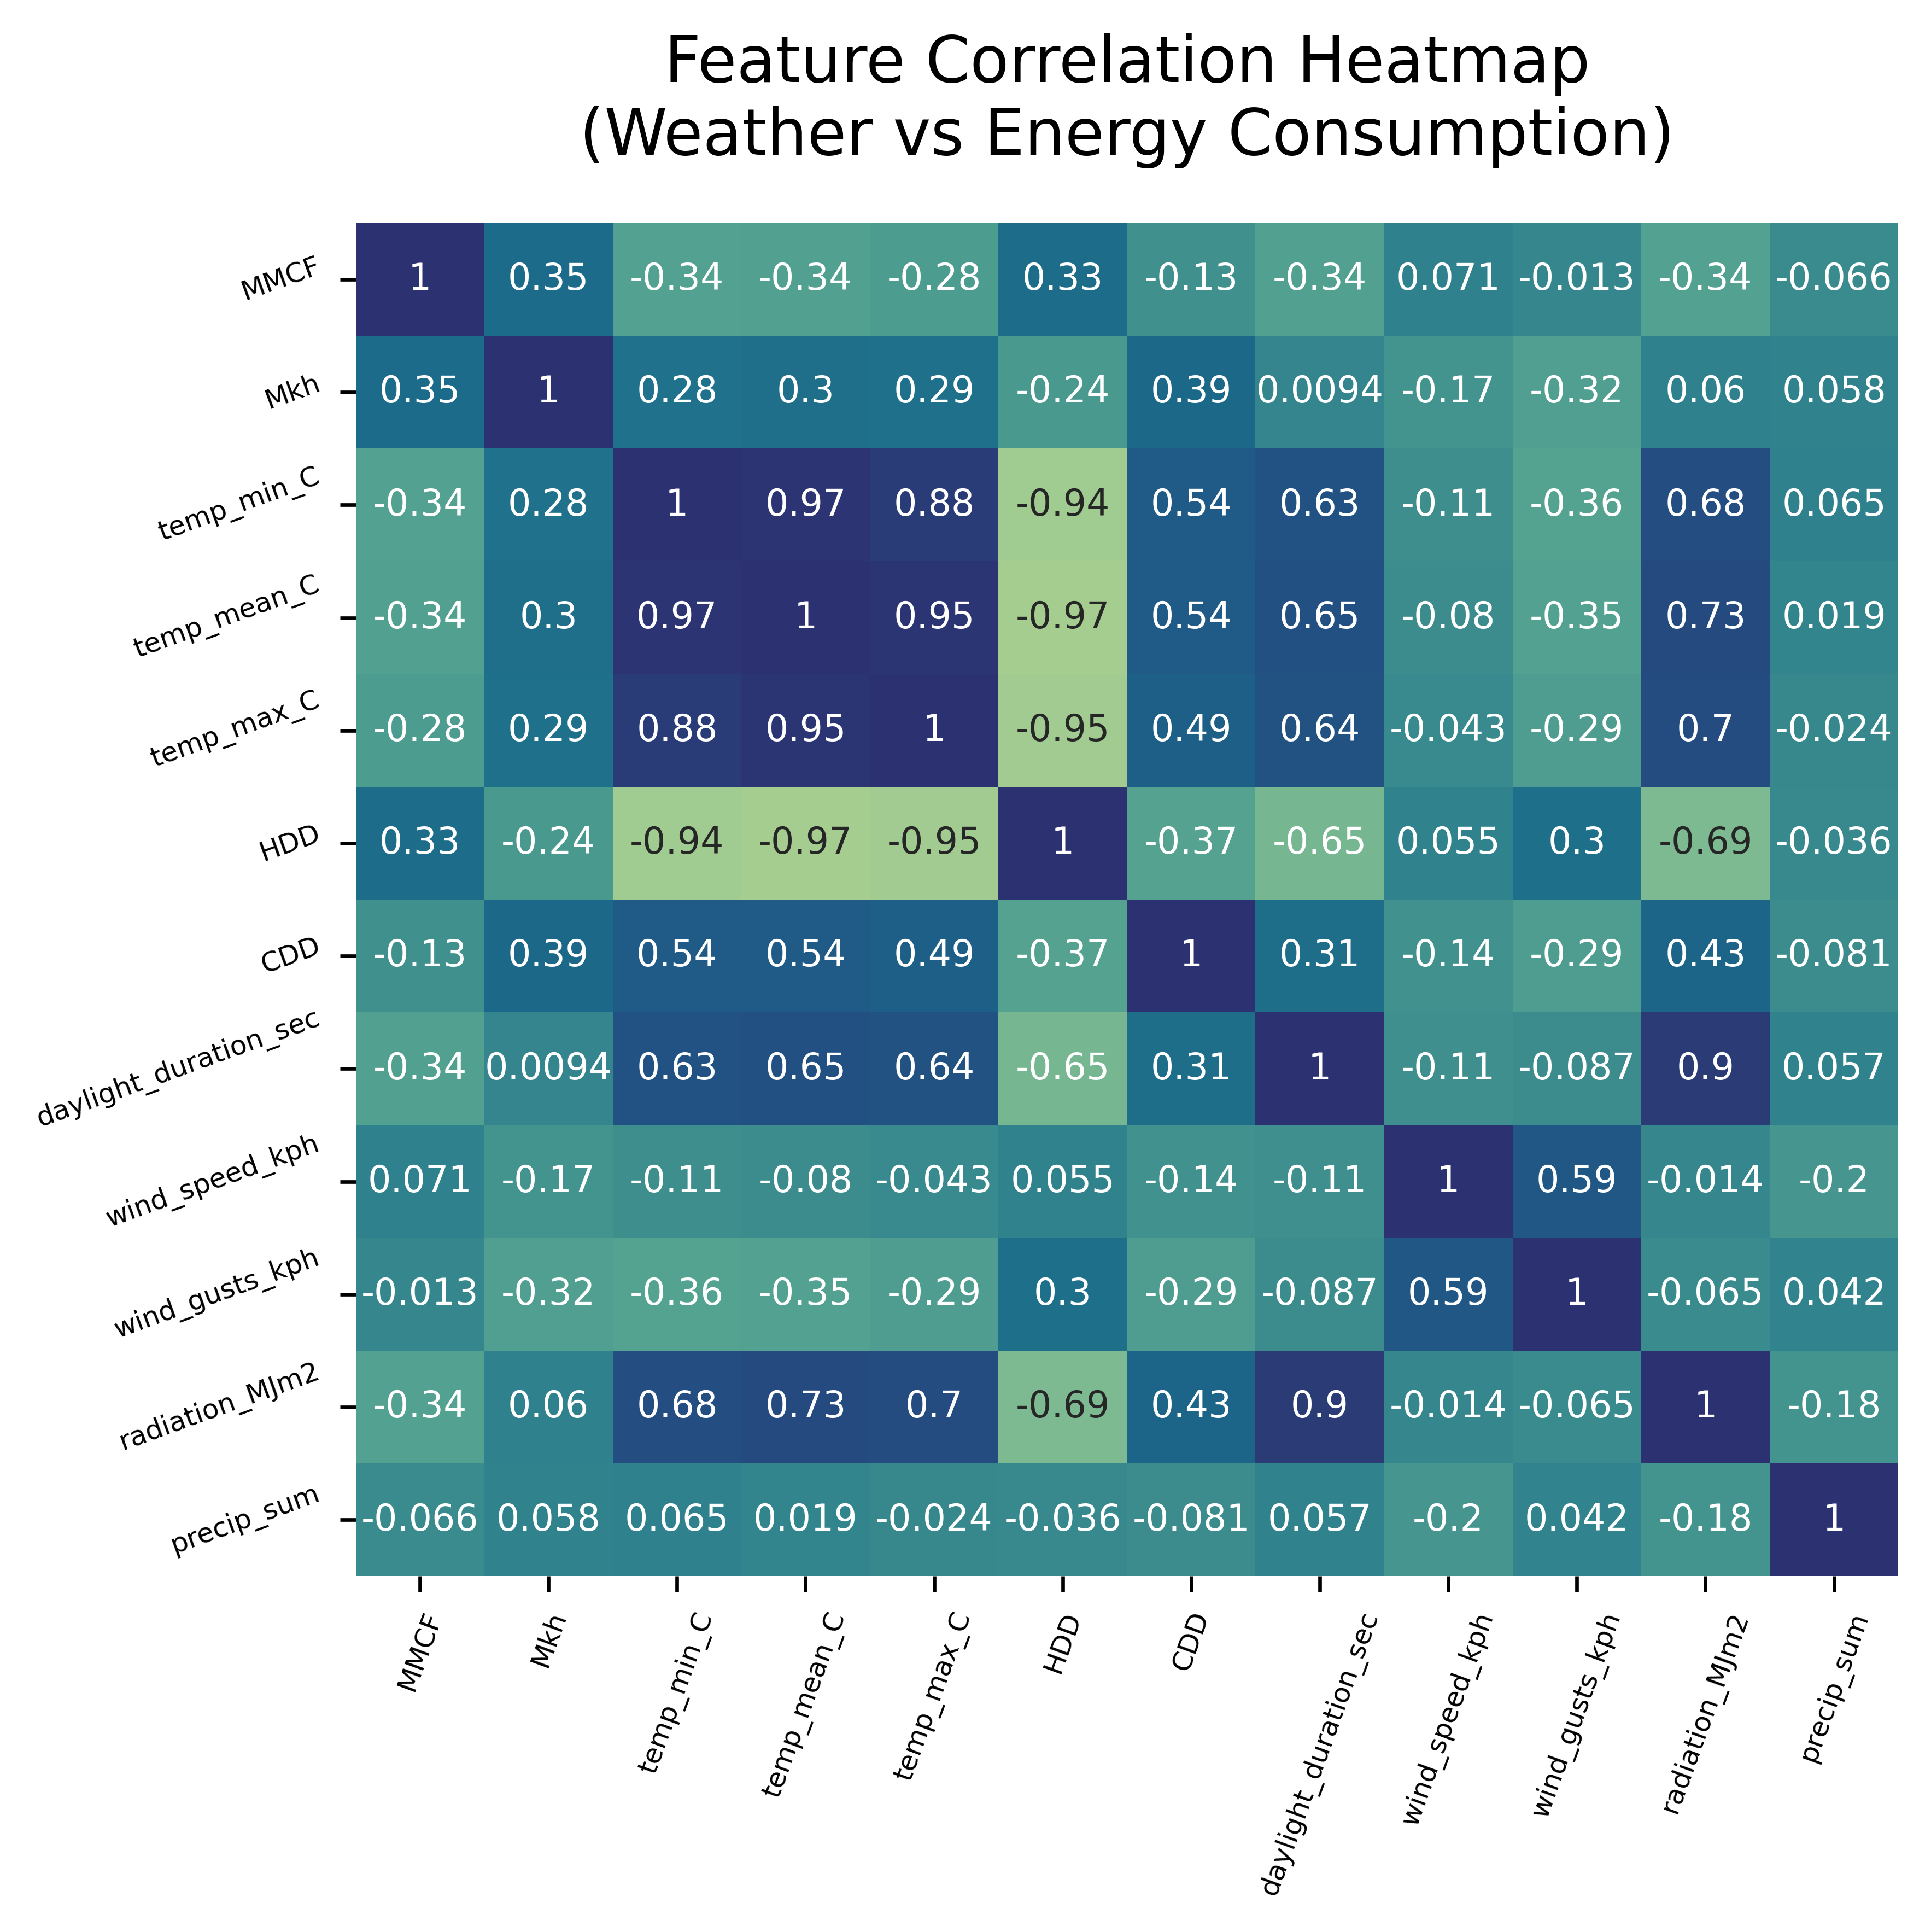
\includegraphics[width=\columnwidth]{corr_heatmap.png}
    \caption{Linear relationships between features}
    \label{fig: 5.3}
\end{figure}
Our correlation heatmap illustrates linear relationships between our target variables (MMCF, Mkh) and all individual weather features falls within (-0.34, 0.35), indicating weak linear relationships. This suggests linear models may have poor performance compared to those which may capture non-linear relationships. Since correlation only captures linear dependence — the true relationship between temperature and energy consumption is likely non-monotonic (high consumption in both very cold and very hot months), meaning the predictive signal may be stronger than these coefficients suggest.\newline
We see a very strong positive correlation between radiation and daylight duration. This is expected, as solar radiation is directly driven by the number of daylight hours.
We see a strong positive correlation between temperature measurements and both daylight duration and radiation, which follows naturally since longer days and greater solar radiation are the primary drivers of seasonal temperature variation.
We also see very strong negative and positive relationships between our engineered heating/cooling degree days (HDD/CDD) and our temperature measurements. This is expected, as HDD and CDD are computed directly from mean daily temperature, which is itself bounded by and correlated with the min/max temperature readings.
Finally, the strong inter-correlation among temperature, radiation, daylight, HDD, and CDD indicates multi-co-linearity within the feature set. While this does not affect tree-based models significantly, it is a consideration when exploring linear models.



%========================================
\section{Data Analysis}

\subsection{Analysis Plan}
Based on observations during data cleaning and exploratory data analysis, some notable results and guidance emerged. These observation serve to inform the strategy of model application. Beginning with linear regression models, scaling, and cross validation, we seek to prove this model outperforms the baseline, avoids overfitting, but more accurate predictions exist. In-line with observations in EDA, we continue to a tree-based random forest models with the intent of proving superior performance to the previous models.  

\subsection{Baseline}
Using linear regression restricted to the date features and outputs, a simple baseline model can be created.
\subsection{Multiple Linear Regression}
Applying multiple linear regression with scaled features assumes linear relationships between features but allows for a straightforward assessment of the relative importance of each feature and evaluation of potential overfitting. Using K-folds cross-validation method (K=5), the model shows no signs of overfitting. This model serves as a secondary baseline given the identification of non-linear relationships in the EDA phase. 

\subsection{Random Forest}
Random Forest was subsequently chosen due to its inherent ability to capture non-linear relationships. Given observations in the EDA phase, the expectation is that Random Forest would outperform linear models. Similar to multiple linear regression, K-folds cross-validation showed no evidence of overfitting and indicated a stable model ready for fitting. Random forest demonstrated marked improvement over the previous models with $R^2$ increasing by 0.21 and 0.04 for natural gas and electricity, respectively; and reducing RMSE to $20\%$ and $43\%$ of that of the linear model for gas and electricity, respectively.

\subsection{Main Results}
\begin{center}
\begin{tabular}{lcc}
\toprule\toprule
Natural Gas\\
\toprule
Model & $R^2$ & RMSE \\
\midrule
Baseline & 0.177 & 11,391 \\
Linear Regression & 0.732 & 6,498\\
Random Forest & 0.987 & 1,404 \\
\toprule \toprule
Electricity\\
\toprule
Model & $R^2$ & RMSE \\
\midrule
Baseline & 0.001 & 2,328 \\
Linear Regression & 0.950 & 518 \\
Random Forest & 0.991 & 224 \\
\bottomrule\bottomrule
\end{tabular}
\end{center}

\textit{Train/Test split: (80\%/20\%)} 

\subsection{Interpretation}

Accurate forecasting of residential energy requirements, both in electricity and natural gas, has broad implications in state-level resource planning and infrastructure investment/development. An accurate, lightweight model trained on easily accessible, open source features with the ability to anticipate energy demand not only showcases interpretability, influence and power; but, also highlights this process can be economical, efficient, and maintainable.  

% =========================================================
\section{Real-World Application}
A model of this nature can be adopted to inform state energy and infrastructure policy by providing data-driven insights into consumption patterns. Professionals in a range of fields can utilize such models to aide in educated decision making as it relates to residential energy consumption and efficiency. In particular, applications in energy generation, power-grid management, and blackout risk assessment represent valuable areas of investment, as improved forecasting enhances reliability and optimizes resource allocation.


% =========================================================
\section{Report Quality and Reproducibility}
\subsection{Running the code}
\begin{itemize}[leftmargin=18pt]
  \item REPO: \href{https://github.com/Duke5t/EnergyConsumption}{Duke5t}
  \item Main file: energy.ipynb
  \item Steps to run: see README.md
  \item Required packages: see requirements.txt
\end{itemize}

% =========================================================
\section{Conclusion and Next Steps}

This paper details a successful approach to predicting both natural gas and electricity residential consumption by state. In addition to accurate predictions, it is shown that a tree based model outperforms linear models given our data. Cooling degree days show a positive correlation with residential electricity consumption but the presence of unexplained variation suggests additional influencing factors. Heating degree days exhibit very strong explanatory power when it comes to residential natural gas consumption. 

\textbf{Next steps:} 
\begin{itemize}
\item Additional data which provides insights into other factors such as quality of residential home energy efficiency by state by month for the previous twenty years would likely prove to be extremely valuable. 
\item Introducing lag variables and time series splits to help identify trends and behavioural patterns.
\item Aggregating weather data from multiple coordinates within each state to better generalize weather summary data.
\end{itemize}
% =========================================================
\section{AI Disclosure}
If you used AI tools (e.g., ChatGPT, Gemini) for coding or writing, disclose it.

\begin{itemize}[leftmargin=18pt]
    \item Chatgpt : Used for API caching and error catching.
    \item Chatgpt : Used to edit visualizations to better fit into the paper.
    \item Chatgpt : Formatting url links into the paper
    \item Chatgpt : Code debugging
\end{itemize}

% =========================================================
\begin{thebibliography}{00}

\bibitem{b1} Energy: https://www.eia.gov/opendata/browser/electricity/retail-sales
\bibitem{b2} Weather : https://open-meteo.com/en/docs
\bibitem{b3} Graff, M., Nock, D. The role of thermostats and human behaviour in residential temperature settings in the USA. Nat Energy 11, 400–414 (2026). https://doi.org/10.1038/s41560-025-01948-w
\end{thebibliography}

\end{document}
